%% bare_jrnl.tex
%% V1.4b
%% 2015/08/26
%% by Michael Shell
%% see http://www.michaelshell.org/
%% for current contact information.
%%
%% This is a skeleton file demonstrating the use of IEEEtran.cls
%% (requires IEEEtran.cls version 1.8b or later) with an IEEE
%% journal paper.
%%
%% Support sites:
%% http://www.michaelshell.org/tex/ieeetran/
%% http://www.ctan.org/pkg/ieeetran
%% and
%% http://www.ieee.org/

%%*************************************************************************
%% Legal Notice:
%% This code is offered as-is without any warranty either expressed or
%% implied; without even the implied warranty of MERCHANTABILITY or
%% FITNESS FOR A PARTICULAR PURPOSE! 
%% User assumes all risk.
%% In no event shall the IEEE or any contributor to this code be liable for
%% any damages or losses, including, but not limited to, incidental,
%% consequential, or any other damages, resulting from the use or misuse
%% of any information contained here.
%%
%% All comments are the opinions of their respective authors and are not
%% necessarily endorsed by the IEEE.
%%
%% This work is distributed under the LaTeX Project Public License (LPPL)
%% ( http://www.latex-project.org/ ) version 1.3, and may be freely used,
%% distributed and modified. A copy of the LPPL, version 1.3, is included
%% in the base LaTeX documentation of all distributions of LaTeX released
%% 2003/12/01 or later.
%% Retain all contribution notices and credits.
%% ** Modified files should be clearly indicated as such, including  **
%% ** renaming them and changing author support contact information. **
%%*************************************************************************


% *** Authors should verify (and, if needed, correct) their LaTeX system  ***
% *** with the testflow diagnostic prior to trusting their LaTeX platform ***
% *** with production work. The IEEE's font choices and paper sizes can   ***
% *** trigger bugs that do not appear when using other class files.       ***                          ***
% The testflow support page is at:
% http://www.michaelshell.org/tex/testflow/



\documentclass[journal]{IEEEtran}
\usepackage[brazilian]{babel}
\usepackage[utf8]{inputenc}
\usepackage[T1]{fontenc}

\usepackage{algorithm}
\usepackage{algpseudocode}
\usepackage{listings}
\usepackage{float}
\usepackage{color}

\floatname{algorithm}{Código}
\algrenewcommand\algorithmicfunction{\textbf{function}}
\algrenewtext{EndFunction}{\algorithmicend}
\algrenewtext{EndIf}{\algorithmicend}


\definecolor{mygreen}{rgb}{0,0.6,0}
\definecolor{mygray}{rgb}{0.5,0.5,0.5}
\definecolor{mymauve}{rgb}{0.58,0,0.82}

\lstset{ %
  backgroundcolor=\color{white},   % choose the background color; you must add \usepackage{color} or \usepackage{xcolor}; should come as last argument
  basicstyle=\footnotesize,        % the size of the fonts that are used for the code
  breakatwhitespace=false,         % sets if automatic breaks should only happen at whitespace
  breaklines=true,                 % sets automatic line breaking
  % captionpos=a,                    % sets the caption-position to bottom
  % commentstyle=\color{mygreen},    % comment style
  deletekeywords={...},            % if you want to delete keywords from the given language
  escapeinside={\%*}{*)},          % if you want to add LaTeX within your code
  extendedchars=true,              % lets you use non-ASCII characters; for 8-bits encodings only, does not work with UTF-8
  % frame=single,	                   % adds a frame around the code
  keepspaces=true,                 % keeps spaces in text, useful for keeping indentation of code (possibly needs columns=flexible)
  % keywordstyle=\color{blue},       % keyword style
  language=Octave,                 % the language of the code
  morekeywords={*,...},            % if you want to add more keywords to the set
  numbers=left,                    % where to put the line-numbers; possible values are (none, left, right)
  numbersep=-5pt,                   % how far the line-numbers are from the code
  numberstyle=\tiny\color{mygray}, % the style that is used for the line-numbers
  rulecolor=\color{black},         % if not set, the frame-color may be changed on line-breaks within not-black text (e.g. comments (green here))
  showspaces=false,                % show spaces everywhere adding particular underscores; it overrides 'showstringspaces'
  showstringspaces=false,          % underline spaces within strings only
  showtabs=false,                  % show tabs within strings adding particular underscores
  % stepnumber=2,                    % the step between two line-numbers. If it's 1, each line will be numbered
  % stringstyle=\color{mymauve},     % string literal style
  % tabsize=2,	                   % sets default tabsize to 2 spaces
  title=\lstname                   % show the filename of files included with \lstinputlisting; also try caption instead of title
}



% *** GRAPHICS RELATED PACKAGES ***
%
\ifCLASSINFOpdf
  \usepackage[pdftex]{graphicx}
  % declare the path(s) where your graphic files are
  \graphicspath{{./img/}}
  % and their extensions so you won't have to specify these with
  % every instance of \includegraphics
  \DeclareGraphicsExtensions{.pdf,.jpg,.jpeg,.png}
\else

\fi

\hyphenation{op-tical net-works semi-conduc-tor}


\begin{document}

\title{Micro-serviços}

\author{Willian Marques Freire e
        Munif Gebara Junior% <-this % stops a space
\thanks{Faculdade de Filosofia Ciências e Letras de Mandaguari é uma fundação
situada em Mandaguari no Paraná região sul brasileira,
na rua Rene Taccola, 152 - Centro Site: (see http://www.fafiman.br/index.html).}% <-this % stops a space
\thanks{Artigo realizado em 2017.}}

\markboth{IoT - Micro-serviços,~Vol.~1, No.~1, Julho~2017}%
{Shell \MakeLowercase{\textit{et al.}}: Bare Demo of IEEEtran.cls for IEEE Journals}

% make the title area
\maketitle

% As a general rule, do not put math, special symbols or citations
% in the abstract or keywords.
\begin{abstract}
The abstract goes here.
\end{abstract}

% Note that keywords are not normally used for peerreview papers.
\begin{IEEEkeywords}
Microservice, Micro-serviço, Eureka.
\end{IEEEkeywords}


\IEEEpeerreviewmaketitle

\section{Introdução}

\IEEEPARstart{M}{icro serviços} é um novo paradigma que influecia diretamente o modo em que são desenvolvidas, e distribuídas as aplicações. Há certas características relacionadas à sua organização, à capacidade de negócio independentes, ao deploy automatizado, à inteligência e controle descentralizado de liguagens e de dados \cite{JamesLewis}. Em uma publicação feita por Sampaio \cite{CleutonSampaio}, o mesmo definiu através de estudos que Micro-serviços são componentes de alta coesão, baixo acoplamente, autônomos e independentes, que representa um contexto de negócio de uma aplicação.

Para exemplificação sobre a motivação do uso de micro-serviços, pode-se citar os sistemas ERP (Enterprise Resource Planning ou sistemas para Planejamentos de Recursos Empresariais), que são desenvolvidos para cuidar de setores empresariais, desde o financeiro, recursos humanos, produção, estoque, dentre outros. Em um sistema para Planejamento de Recursos Empresariais, todas as funcionalidades do mesmo são agrupadas dentro deste grande sistema, fazendo com que seja uma aplicação monolítica, ou seja, uma aplicação feita em somente uma unidade.

Por consequência, um dos principais pontos negativos, é que se houver um grande ponto de falha em algum módulo do sistema, isto poderá afetar a aplicação inteira, incluindo funcionalidades não relacionadas com o mesmo. Outro ponto negativo, é a base de código fonte, que se torna exponencialmente extensa de acordo com o tempo de desenvolvimento, tornando assim, novos membros do projeto improdutivo durante algum tempo, já que a complexida do código é bem maior \cite{AdrianoAlmeida}.

Um fato que ocorreu no ano de 2014, foi que o Docker (\emph{container} portátil padronizado) começou a ser utilizado amplamente pela comunidade de desenvolvedores. Uma razão importante para sua utilização generalizada que Adrian (Membro e fundados da eBays Research Labs) observa, é sua portabilidade e aumento na velocidade com \emph{container} de aplicações, que entregava algo em minutos ou horas e passou a entregar em segundos \cite{CristianoDiedrich}. Na figura \ref{fig:utilizacao-docker} é apresentado sua utilização entre os anos 2012 e 2016.

\begin{figure}[h]
\centering
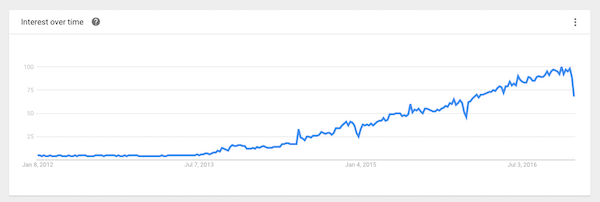
\includegraphics[height=1.1in]{docker}
\caption{Gráfico de utilzação do docker entre os anos 2012 e 2016.}
\label{fig:utilizacao-docker}
\end{figure}

Semelhantemente, a velocidade de desenvolvimento e implantação de um micro-serviço, permite e incentiva a implementação e estudo dos mesmos. Segundo Adrian micro-serviços possuem também outras características em comum, como implantação com pouca frequência, novas versões implantadas automaticamentes, orquestração de uso geral não é necessário (uma vez que, sistemas inteiros são implantados com todas as partes ao mesmo tempo), arquiteturas utilizam centenas de micro-serviços, e cada publicação, é altamente customizada \cite{JanStenberg}.

Sendo assim, implantar a Arquitetura de Micro-serviços em empresas, irá proporcionar diferentes benefícios para a estrutura de negócio como, usufruir de liberdade maior para o desenvolvimento de serviços de modo independente, implantar aplicações automaticamente através de ferramentas de integração contínua (como Hudson, Jenkins e outras), possibilitar utilização de códigos escritos em linguagens diferentes para diferentes serviços, facilitar a ampliação e integração de micro-serviços com serviços terceirizados (atráves de APIs), organizar o código em função de capacidades de negócio, dando assim, mais visão das ofertas e necessidades dos clientes. Dentre todos os benefícios citados, também é possível fazer o gerenciamento de falhas, visto que, o particionamento favorece uma visão mais detalhada de cada serviço, o que significa que se um serviço venha a falhar, os outros continuarão funcionando \cite{RicardoPeloi}.

Este trabalho têm por objetivo, preencher a lacuna a respeito do desenvolvimento de uma simples estrutura para micro-serviços, fazendo com que, utilizando-se de ferramentas existentes, seja fácil a criação da mesma. Durante este trabalho, serão criados micro-serviços, que posteriormente abrirão possibilidades para integração entre eles e outros serviços existentes. O mesmo está organizado entre uma revisão biliográfica sobre o assunto, uma parte com desenvolvimento dos micro-serviços, e a apresentação de resultados pouco antes da conclusão.

\hfill 13 de Maio de 2017

\subsection{Revisão bibliográfica}

Segundo dados de Chris Richardson \cite{ChrisRichardson}, diversas empresas estão utilizando micro-serviços, dentre as citadas estão: Comcast Cable, Uber, Netflix, Amazon, Ebay, SoundCloud, Karma, Groupon, Hailo, Gilt, Zalando, Lending Club, AutoScout24.
Os problemas associados ao desenvolvimento de software em larga escala ocorreram em torno da década de 1960. Posteriormente, na década de 1970 viu-se um enorme aumento de interesse da comunidade de pesquisa, para o design de software em suas aplicações e no processo de desenvolvimento. Nesta década, o design foi muitas vezes considerado como uma atividade não associada com a implementação em si, e portanto requerendo um conjunto especial de notações e ferramentas. Por volta da década de 1980, a integração do design nos processos de desenvolvimento contribuiu para uma fusão parcial dessas duas atividades, tornando assim mais difícil fazer distinções puras.

Da mesma forma, as referências ao conceito de arquitetura de software também começaram a aparecer década de 1980. No entanto, uma base sólida sobre o tema foi estabelecida apenas em 1992, por Perry Wolf (autor do livro “Foundations for the study of software architecture"). Sua definição de arquitetura de software era distinta do design de software, e desde então tem-se gerado uma grande comunidade de pesquisadores estudando as aplicações práticas da arquitetura de software com base em micro-serviços, permitindo dddassim que os conceitos sejam amplamente adotados pela indústria e pela academia.

O advento e a difusão da orientação a objetos, a partir dos anos 80 e, em particular, a década de 1990, trouxe sua própria contribuição para o campo da Arquitetura de Software. O clássico por Gamma et ai. abrange a concepção de software orientado a objetos e como traduzi-lo em código que apresenta uma coleção de soluções recorrentes, chamados padrões. Esta ideia não é nova nem exclusiva à Engenharia de Software, mas o livro é o primeiro compêndio a popularizar a idéia em grande escala. Na era pré-Gamma, os padrões para soluções orientada a objetos já estavam sendo utilizado. Um exemplo típico de um padrão de projeto arquitetônico em programação orientada a objetos, é o Model-View-Controller (MVC), que tem sido um dos insights seminais no desenvolvimento precoce de interfaces gráficas de usuário \cite{nicoladragonietal}.

Cerca de sete anos atrás a empresa Netflix (provedora global de filmes e séries de televisão via streaming - distribuição de dados, geralmente de multimídia em uma rede através de pacotes) começou a migrar suas aplicações legadas para uma arquitetura baseada em APIs, (Interface de programação de aplicativos) hospedadas na nuvem (local para armazenamento de dados online) da Amazon (empresa transnacional de comércio electrónico dos Estados Unidos com sede em Seattle), influenciando assim, o crescimento de uma ideologia na área de desenvolvimento de softwares que foi batizada pelo nome de “micro-serviço”.

Pouco antes, uma investigação realizada pela empresa Cisco (Companhia sediada em San José, Califórnia, Estados Unidos da América) em 2016 revela que, apesar de toda a euforia sobre a Internet das Coisas, o consumo de de vídeo via internet gera 63\% do tráfego global. A expectativa é que essa marca chegue a 79\% até 2020 e o tráfego de dados gerado por vídeos em resolução Ultra HD subirá de 1.6\% para 20.7\% do total em 2020. Um levantamento realizado pela Cisco VNI Mobile em 2016 também mostra que os dispositivos IoT mais simples, geram uma quantidade de dados equivalentes a 7 vezes o que é produzido por um celular comum (não um smartphone). Demandando pouco das redes de telecomunicações, os dispositivos IoT não representarão um grande pessoa para os provedores de infraestrutura na América Latina \cite{idc2017}. 

A fim de informação sobre a utlização de internet nos últimos anos, segundo o relatório “The State of Internet” de 2016, da Akamai (Empresa de Internet americana, sediada em Cambridge, Massachusetts), o país melhor colocado na faixa de redes com banda igual ou maior a 15 Mb/s é o Chile - 4,4\% de seus serviços de Internet atingem essa marca. Entretanto, para chegar a essa posição, o Chile investiu pesadamente entre 2014 e 2015, conseguindo crescer 150\% de um ano para outro. O Uruguai fica logo abaixo, com 4,1\% de sua Internet na faixa dos 15 Mb/s. Atualmente no Brasil, somente 1,1\% dos serviços atingem esta marca.

Na arquitetura de micro-serviços, quando é feito a implantação ou atualização dos mesmos, não é afetado outros serviços, e cada micro-serviço pode ser desenvolvido em uma linguagem diferente. Governança granular também é possível para cada micro-serviço, já que o mesmo não tem dependência com outros, e pode ser monitorado e coreografado separadamente. Essa arquitetura descentraliza o gerenciamento de dados, uma vez que cada micro-serviço pode armazenar seus dados de uma maneira que se adapte a ele, e são mais resistentes do que as aplicações tradicionais, devido ao fato de que uma única aplicação pode ser retirada de um monte de aplicações, considerando que são independentes uns dos outros.

\subsubsection{Tecnologias para gerenciamento de Micro-serviços}
Neste trabalho foi utilizado diversas tecnologias para desenvolvimento dos micro-serviços. A principal utilizada que é utilizado para registro centralizado das aplicações, é a tecnologia da Netflix \emph{Service Discovery (Eureka)}. Existem outras bibliotecas que podem trabalhar em conjunto com o Eureka, e serão utilizadas neste trabalho, algumas são: Circuit Breaker (Hystrix), Intelligent Routing (Zuul) and Client Side Load Balancing (Ribbon). 

\subsubsection{Zuul}
Zuul é a ''porta da frente'' para todas as requisições de dispositivos e sites para o \emph{back-end}. O mesmo foi construído para permitir roteamento dinâmico, monitoramento, resiliência e segurança. O Zuul foi desenvolvido pela Netflix pelo fato de que, o volume e a diversidade do tráfego da API do mesmo, resultam em problemas de produção, surgem rapidamente e sem aviso prévio, e a empresa necessitava de um sistema que permita os mesmos mudarem rapidamente o comportamento e reagir a estas situações. O Zull utiliza diferentes tipos de filtros, que permitem aplicar rapidamente funcionalidades aos serviços de ponta. 

Em suma, esses filtros ajudam a executar as seguintes funções: Autenticação e segurança, identificação de requisitos de autenticação para cada recurso, negação de solicitações indesejadas, insights e monitoramento, rastreamento de dados significativos e estatísticas, a fim de dar uma visão precisa da produção, roteamento dinâmico, encaminhamento dinâmico solicitações para diferentes clusters de backend conforme necessário, \emph{stress Testing}, aumento gradual de tráfego para um cluster, a fim de avaliar o desempenho, \emph{load Shedding}, alocação de capacidade para cada tipo de solicitação e liberação de pedidos que excedem o limite, manipulação de resposta estática e construção de respostas diretamente na ponta ao invés de encaminhá-las para um cluster interno.
Dentre os vários componentes que integram a biblioteca do Zuul, estão: Zuul-core que contém funcionalidades a fim de compilar e executar filtros, Zuul-simple que demonstra como construir um aplicativo com zuul-core e Zuul-netflix que adiciona componentes Netflix utilizando Ribbon para solicitações de roteamento \cite{netflix2016Zuul}.


\subsubsection{Ribbon}
Ribbon oferece suporte à comunicação entre processos na nuvem, e inclui balanceadores de carga desenvolvidos pela netflix. A tecnologia citada fornece os seguintes recursos: regras de balanceamento de carga múltiplas e conectáveis, integração com a descoberta de serviços, resiliência de falhas incorporada e clientes integrados com balanceadores de carga. O Ribbon é composto pelos seguintes projetos: \emph{Ribbon-core} que inclui definições de interface e balanceamento de carga e cliente, implementações de balanceador de carga comuns, integração de cliente com balanceadores de carga e fábrica de clientes. \emph{Ribbon-eureka} que inclui implementações do balanceador de carga com base no \emph{Eureka-client} (biblioteca para registro e descoberta de serviços). \emph{Ribbon-httpclient} que inclui a implementação de balanceamento de carga baseada em JSR-311 \cite{netflix2016Ribbon}.

\subsubsection{Hystrix}
Em um ambiente distribuído, inevitavelmente algumas das muitas dependências de serviços falharão, e esta biblioteca ajuda a controlar as interações entre serviços distribuídos, adicionando tolerância de latência e lógica de tolerância a falhas. O mesmo faz isso isolando pontos de acesso entre os serviços, interrompendo falhas em cascata através deles, todas as quais melhoram a resiliência geral do sistema. Atualmente, dezenas de bilhões de threads isoladas e centenas de bilhões não isoladas, são executadas utilizando o Hystrix todos os dias na Netflix. Isso resulta em uma melhoria dramática no tempo, atividade e resiliência das aplicações. Hystrix é um projeto desenvolvido também para proteger e controlar a latência e falhas, de dependências acessadas por meio de bibliotecas de terceiros, monitoramento em tempo real, alertas e controle operacional. Quando se trata de micro-serviços, os mesmos contém dezenas de dependências com outros serviços, o que ocasiona que se um deles falhar, e o mesmo não estiver isolado destas falhas externas, corre o risco de também ser afetado. Como exemplo, um aplicativo que dependa de 40 serviços, em que cada serviço tem 99,99\% de disponibilidade, pode se esperar: 99,99 \^ 40 = 99,6\% de tempo de atividade, 0.4\% de 1 bilhão de falhas resulta em 4 milhões de falhas. Mesmo que pequena a possibilidade de falha, se somar a quantidade de micro-serviços ao tempo de indisponibilidade que pode surgir por pequenas falhas, o problema pode ser facilmente escalável fazendo com que assim serviços importantes fiquem até mesmos horas indisponíveis. Quando toda a aplicação está funcionando e configurada de maneira correta, o fluxo de solicitações ocorrer conforme a figura \ref{fig:hystrix-overtime}.

\begin{figure}[h]
\centering
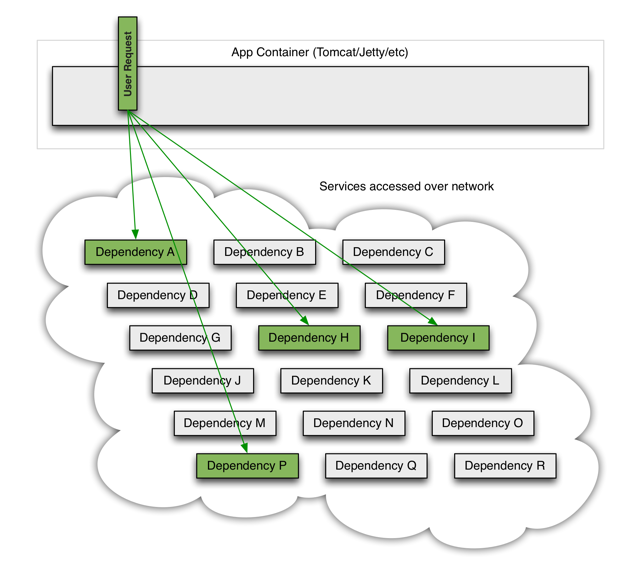
\includegraphics[height=6.2cm]{figura3}
\caption{Wiki Hystrix (Internet Overtime) - 2015).}
\label{fig:hystrix-overtime}
\end{figure}

Quando um dos muitos serviços se torna latente, ele pode bloquear toda a solicitação do usuário, conforme apresentado na figura \ref{fig:hystrix-dimensions-scaling}.

\begin{figure}[h]
\centering
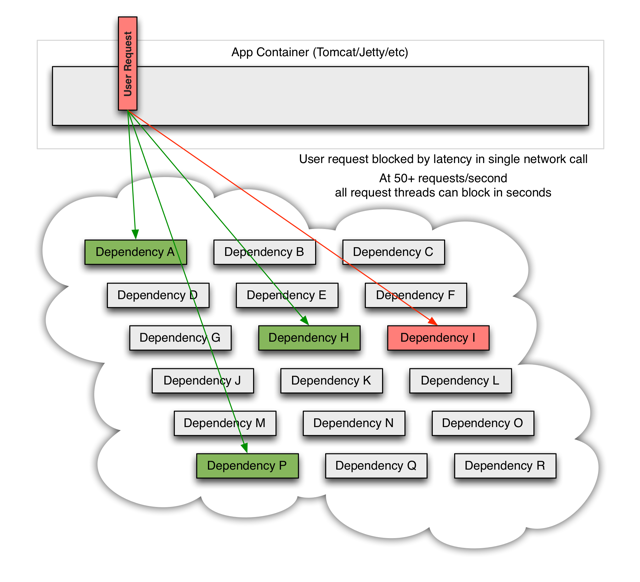
\includegraphics[height=6.2cm]{figura4}
\caption{Wiki Hystrix (3 dimensions to scaling) - 2015).}
\label{fig:hystrix-dimensions-scaling}
\end{figure}

Com tráfego de alto volume, uma única dependência com latência excessiva, pode fazer com que todos os recursos fiquem saturados em segundos. Cada ponto em um aplicativo que atinge a rede, ou em uma biblioteca cliente que pode resultar em solicitações de rede, é uma fonte de falha potencial. Esses aplicativos também podem resultar em latências entre os serviços, causando ainda mais falhas em cascata em todo a aplicação, conforme a figura \ref{fig:hystrix-container}.

\begin{figure}[h]
\centering
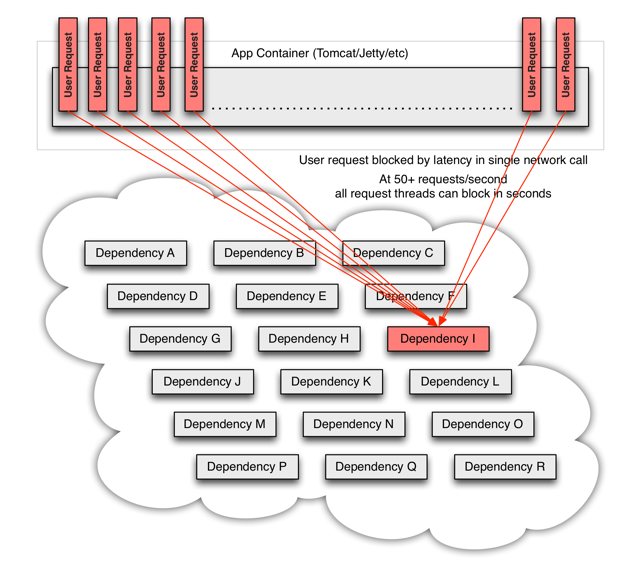
\includegraphics[height=6.2cm]{figura5}
\caption{Wiki Hystrix (Container) - 2015).}
\label{fig:hystrix-container}
\end{figure}

A biblioteca Hystrix subjaz os seguintes princípios de design: impedir que qualquer dependência única utilize todas as threads de usuários de um container (como Tomcat) desperdiçando carga do sistema, fornecer soluções sempre que possível para proteger os usuários contra falhas, utilizar técnicas de isolamento para limitar o impacto de qualquer dependência, otimizar o tempo de descoberta através de métricas, monitoramento e alertas em tempo real, otimizar o tempo de recuperação por meio de propagação de baixa latência de alterações de configuração e, oferecer suporte para alterações de propriedade dinâmicas na maioria dos aspectos do Hystrix, o que permite fazer modificações operacionais em tempo de execução com loops de realimentação de baixa latência, protegendo contra falhas em toda a execução do cliente, não apenas no tráfego da rede. (Hystrix, 2015)

\subsubsection{Eureka + Spring Cloud}
Spring Cloud fornece integrações Netflix OSS para Spring Boot por meio de auto-configuração, e vinculação ao Spring Environment e outros padrões de programação Spring. Dentre os produtos Spring Cloud encontra-se, os clientes Eureka ou Service Discovery, que é um dos princípios fundamentais de uma arquitetura baseada em micro-serviços. Configurar um micro-serviço é trabalhoso, pois envolve diversas técnicas de descoberta e registro de serviços, e com o Service Discovery da Netflix, torna-se eficiente este trabalho pois com poucas anotações Java consegue-se criar uma aplicação simples Eureka. 

Eureka também vem com um componente de cliente baseado em Java, o cliente Eureka, que torna as interações com o serviço muito mais fácil. O cliente também tem um balanceador de carga incorporado, que faz balanceamento de carga \emph{round-robin} (Algoritmos simples de agendamento e escalonamento de processos) básico. Quando um cliente se registra no Eureka, o mesmo fornece metadados como host e porta, dentre outras informações que podem ser encontradas na documentação. Se o registro falhar durante a configuração, a instância da aplicação é removida do registro. Em resumo, o Eureka é um serviço baseado em REST (Representational State Transfer), que é utilizado principalmente na AWS (Amazon Web Services), para localizar serviços com a finalidade de balanceamento de carga, e failover (tolerância a falhas) de servidores de camada intermediária. 

Semelhantemente, a Amazon possui um produto chamado AWS ELB (Amazon Web Services Elastic Load Balancer), que é uma solução de balanceamento de carga para serviços de ponta, expostos ao tráfego web do usuário final, e a diferença entre o mesmo e o produto da Netflix, é que o Eureka preenche a necessidade de balanceamento de carga médio. Embora teoricamente pode-se colocar serviços de nível intermediário junto com o AWS ELB, no EC2 classic (Elastic Compute Cloud), pode-se expor à rede externa, e perder toda a utilidade dos grupos de segurança AWS. O AWS ELB  também possui uma solução de balanceamento de carga em proxy (servidor intermediário para requisições entre cliente e servidor final) tradicional, enquanto no Eureka, o balanceamento ocorre no nível da instância, servidor e host. As instâncias do cliente sabem todas as informações sobre quais aplicações precisam conversar.

Na Netflix, além de desempenhar um papel crítico no balanceamento de carga de nível médio, o Eureka é utilizado para os seguintes fins: implementações com Netflix Asgard, um serviço para fazer atualizações de serviços de forma rápida e segura, registro e exclusão de instâncias e transporte de metadados específicos de aplicativos adicionais sobre serviços. Dentre os motivos para utilizar o Eureka está o fato de que, o mesmo provê uma solução para balanceamento de carga round-robin simples, e quando não pode-se expor o tráfego das aplicações externamente com o AWS ELB, o Eureka resolve este problema.

Sendo assim, com o Eureka a comunicação é transparente, pois o mesmo fornece informações sobre os serviços desejados para comunicação, mas não impõe quaisquer restrições sobre o protocolo ou método de comunicação. Exemplificando, pode-se utilizar o Eureka para obter o endereço do servidor destino e utilizar protocolos como thrift, http(s) ou qualquer outro mecanismos RPC (Remote Procedure Call) que permite fazer conexões ou chamadas por espaço de endereçamento de rede. 

\subsubsection{Modelo Arquitetural Eureka}
O modelo arquitetural implantado na Netflix utilizando o Eureka é descrita na figura \ref{fig:wiki-eureka-est}. Existe um cluster por região que conhece somente instâncias de sua região. Há pelo menos um servidor Eureka por zona para lidar com falhas da mesma. Os serviços se registram e, em seguida, a cada 30 segundos enviam os chamados ''batimentos cardíacos'' ou requisições para renovar seus registros. Se o cliente não renovar o registro, ele é retirado do servidor em cerca de 90 segundos. As informações de registro e renovações são replicadas para todos as conexões no cluster. Os clientes de qualquer zona podem procurar as informações do registro para localizar seus serviços que podem estar em qualquer zona e fazer chamadas remotas.

Para serviços não baseados em Java, têm-se a opção de implementar a parte do cliente, utilizando o protocolo REST desenvolvido para o Eureka ou executar um ''side car'' que é uma aplicação Java com um cliente embutido Eureka, que manipula os registros e conexões. Quando se trabalha com serviços em nuvem, pensar em resiliência se torna ímprobo. Eureka se beneficia dessa experiência adquirida, e é construído para lidar com falha de um ou mais servidores do mesmo.

\begin{figure}[h]
\centering
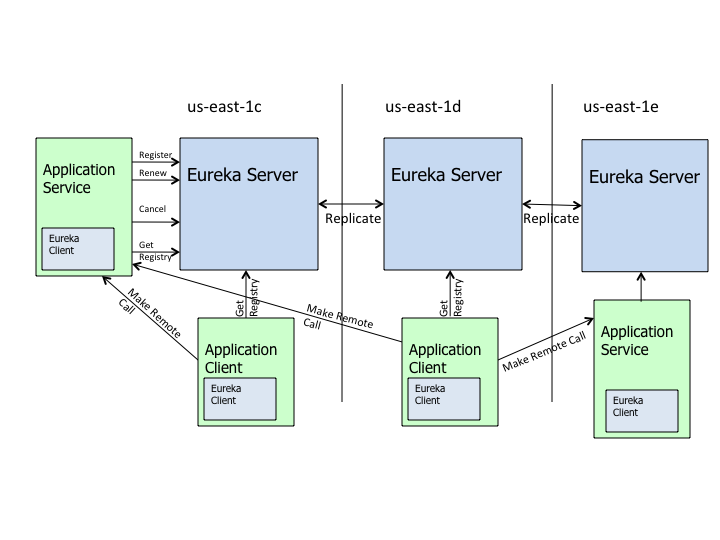
\includegraphics[height=6.2cm]{figura6}
\caption{Wiki Eureka - 2015).}
\label{fig:wiki-eureka-est}
\end{figure}
 

\subsection{Desenvolvimento}

\subsection{Iniciando com Eureka Client}

Este trabalho tem por objetivo o a pesquisa e desenvolvimento de uma estrutura de micro-serviços. Como o projeto será baseado em Java, inicialmente será criado um projeto que utilizará maven, para gerenciamento de dependências, e o Eureka Client para descoberta de serviços. Após a criação de um projeto utilizando Maven, será incluso o groupId org.springframework.cloud e o artifactId spring-cloud-starter-eureka no arquivos de configuração das dependências.

Como resultado, quando um cliente se registra com o Eureka, ele fornece meta-dados sobre si, indicador de estado ou saúde, página inicial, dentre outros. O Eureka recebe mensagens heartbeat (disponibilidade) de cada instância pertencente a um serviço, e se algum heartbeat falhar, a instância é removido do registro.
Para inicializar um projeto com Eureka Client, será utilizado algumas anotações Java fornecidas pelo Eureka descritas a seguir: @Configuration, para utilizar recursos do projeto Spring Config, para facilitar configurações de projetos Spring baseado em Java, @ComponentScan para buscar componentes em pacotes java, @EnableAutoConfiguration para ativar as configurações automáticas internas, @EnableEurekaClient para ativar a descoberta de serviços do Eureka, @RestController para criar um controlador Rest (Representational State Transfer), @RequestMapping para mapear as rotas da aplicação. As mesmas podem ser visualizadas na figura \ref{alg:eurekainicio}.

\begin{figure}[h]
\centering

\begin{lstlisting}[language=Java]
  @Configuration
  @ComponentScan
  @EnableAutoConfiguration
  @EnableEurekaClient
  @RestController
  public class Application {

      @RequestMapping("/")
      public String home() {
          return "Hello world";
      }

      public static void main(String[] args) {
          new SpringApplicationBuilder
            (Application.class).web(true)
            .run(args);
      }
  }
\end{lstlisting}

\caption{Inicio de utilização do Eureka}
\label{alg:eurekainicio}
\end{figure}

Para que possa surtir efeito na aplicação, é necessário fazer ajustes nas configurações do Eureka, dentro do diretório resources da aplicação Java. Esta configuração é feita dentro de um arquivo Application.yml conforme a figura \ref{alg:configeureka}.

\begin{figure}[h]
\centering

\begin{lstlisting}[language=Java]
  Eureka
   cliente:
     ServiceUrl:
       DefaultZone: 
        http://localhost:8761/eureka/ 
\end{lstlisting}

\caption{Configuração do Eureka}
\label{alg:configeureka}
\end{figure}

Neste arquivo de configuração, encontra-se uma peculiaridade. O DefaultZone é a URL do serviço Eureka para qualquer cliente. O nome do aplicativo padrão (ID de serviço), o host e a porta podem ser acessadas respectivamente pelas variáveis de ambientes: \${spring.application.name} , \${spring.application.name} e \${server.port}.
A anotação Java @EnableEurekaClient faz com que, a aplicação corrente se registre no Eureka, para que assim possa localizar outros serviços.

\subsection{Status e Saúde do serviço}

Com a página de status e os indicadores de integridade de uma instância do Eureka, é possível visualizar informações do serviço. Para acessar os indicadores de saúde, deve-se configurar as rotas padrões de acesso a mesma. Por padrão, o eureka utiliza a conexão do cliente, para determinar se está ativo. Caso não seja utilizado o Discovery Client, não será propagado o status de verificação de integridade atual do serviço. Para que os indicadores de saúde e status da aplicação funcionem corretamente, devem ser feito configurações conforme a figura \ref{alg:figuratres}.

\begin{figure}[h]
\centering

\begin{lstlisting}[language=Java] 
  eureka:
    instance:
      statusPageUrlPath: 
        ${management.context-path}/info
      healthCheckUrlPath: 
        ${management.context-path}/health
    client:
      healthcheck:
        enabled: true
\end{lstlisting}

\caption{Configuração de indicadores de Status}
\label{alg:figuratres}
\end{figure}

Para conseguir utilizar mais recursos e obter mais informações sobre o status da aplicação, a aplicação deve implementar seu próprio controle de integridade que se encontra no pacote com.netflix.appinfo.HealthCheckHandler

\subsection{Alterando o ID da instância Eureka}

Uma instância registrada no Eureka possui seu ID, que identifica o serviço que está no mesmo. O Spring Cloud Eureka fornece o seguinte padrão de configuração: \$\{spring.cloud.client.hostname\}:\$\{spring.application.name\}:
\$\{spring.application.instance\_id:\$\{server.port\}\}. Como exemplo a URL fica da seguinte maneira: myhost:myapp:8080

\subsection{Iniciando com EurekaClient}

O próximo passo para utilizar o Eureka Server para coreografar os micro-serviços, é utlizar o Eureka Client, que pode ser utilizado para descobrir instâncias do mesmo. Para fazer isto utilizando o framework, primeiramente é necessário incluir a dependência do EurekaClient, e criar um método que busque as instâncias registradas no Eureka conforme a \ref{alg:figuraquatro}.


\begin{figure}[h]
\centering

\begin{lstlisting}[language=Java]
  @Autowired
  private EurekaClient discoveryClient;

  public String serviceUrl() {
    InstanceInfo instance = 
      discoveryClient
      .getNextServerFromEureka
        ("STORES", false);
      return instance.getHomePageUrl();
  } 
\end{lstlisting}

\caption{Busca de instâncias}
\label{alg:figuraquatro}
\end{figure}

Não necessariamente é preciso utilizar o EurekaClient. Também pode-se utilizar o DiscoveryClient. A diferença entre os dois, está na maneira de como é utilizado. A mesma pode ser vista na figura \ref{alg:figuracinco}

\begin{figure}[h]
\centering

\begin{lstlisting}[language=Java]
  @Autowired
  private DiscoveryClient discoveryClient;

  public String serviceUrl() {
      List<ServiceInstance> list = 
        discoveryClient.getInstances
          ("STORES");
      if (list != null && list.size() > 0 ) {
          return list.get(0).getUri();
      }
      return null;
  }
\end{lstlisting}

\caption{Busca de instâncias com DiscoveryClient}
\label{alg:figuracinco}
\end{figure}

\subsection{Performanece de registro no Eureka}

Registrar um serviço no Eureka pode ser considerado um pouco lento, pelo fato de que, ser uma instância também envolve um heartbeat periódico para o registro, com duração padrão de 30 segundos. Um serviço não estará disponível para descoberta por clientes, enquanto uma intância tenha todos os metadados em seu cache local. Para alterar o período em que isto ocorre, pode ser configurado através da propriedade eureka.instance.leaseRenewalIntervalInSeconds. Entretanto, em produção, não deve ser alterado este padrão pelo fato de que, existem alguns cálculos internos do Eureka, que fazem suposições de renovação de locação.

\subsection{Zonas Eureka}

Primeiramente, para se configurar uma zona Eureka, é necessário ter certeza de que existem servidores Eureka implantados em cada zona e que eles são pares uns dos outros. Em seguida, precisa-se informar em qual zona o mesmo está. Para fazer isto será utilizado a propriedade metadataMap. E isto pode ser feito conforme a figura \ref{alg:figuraseis}.

\begin{figure}[h]
\centering

\begin{lstlisting}[language=Java]
  eureka.instance.metadataMap.zone = zone1
  eureka.client.preferSameZoneEureka = true
\end{lstlisting}

\caption{Compilação do firmware}
\label{alg:figuraseis}
\end{figure}

\subsection{Primeiros passos com Eureka Server}

Como este projeto é baseado em Java no backend, e utiliza maven como gerenciador de dependências, será incluso nas configurações de dependências Maven o groupId org.springframework.cloud e o artifactId spring-cloud-starter-eureka-server. Com esta dependência adicionada, será possível utilzar o Eureka Server.

Após adicionar esta dependência, será criado a classe principal, que se encarregará de iniciar a aplicação Eureka Server. Utilizando-se da anotação @EnableEurekaServer fornecida pelo framework, e seguindo o padrão utilizado no Eureka Client para iniciar a aplicação, é possível ver um resultado. Um exemplo de código pode ser na figura \ref{alg:figurasete}.

\begin{figure}[h]
\centering

\begin{lstlisting}[language=Java]
  @SpringBootApplication
  @EnableEurekaServer
  public class Application {
    public static void main(String[] args) {
        new SpringApplicationBuilder
          (Application.class).web(true)
          .run(args);
    }
  }
\end{lstlisting}

\caption{Código inicial Eureka Server}
\label{alg:figurasete}
\end{figure}

\subsection{Modo Autônomo}

A combinação entre o cliente e servidor Eureka, e as pulsações para verificação de disponibilidade entre os mesmos, tornam o servidor Eureka resiliente à falhas, contanto que haja algum tipo de monitoramento para mantê-lo funcionando. No modo autônomo, pode-se prefirir desativar o comportamento padrão do lado do cliente, para que ele não continue tentado alcançar seus pares caso haja falha. Para isto será feito diversas configurações como pode ser visto na figura \ref{alg:figuraoito}.

\begin{figure}[h]
\centering

\begin{lstlisting}[language=Java]
  server:
    port: 8761

  eureka:
    instance:
      hostname: localhost
    client:
      registerWithEureka: false
      fetchRegistry: false
      serviceUrl:
        defaultZone: 
          http://${eureka.instance.hostname}
          :${server.port}/eureka/
\end{lstlisting}

\caption{Confiugração Eureka Server}
\label{alg:figuraoito}
\end{figure}

Acima foi apresentado as seguintes configurações: port que configura a porta em que será instalado a aplicação, hostname para identificar o nome do host, registerWithEureka que indica se a própria aplicação do Eureka se registrará em si mesma, e fetchRegistry que diz se o Eureka buscará registros associados a eles que ainda estão executando, porém ainda não registradas no Eureka.
Com o Eureka, os registros podem ser ainda mais resistentes e disponíveis, executando várias instâncias e pedindo-lhes para se registrarem uns com os outros. Tudo o que precisa para fazê-lo é configurar o serviceUrl dos pares, conforme a figura \ref{alg:figuranove}

\begin{figure}[h]
\centering

\begin{lstlisting}[language=Java]
  ---
  spring:
    profiles: peer1
  eureka:
    instance:
      hostname: peer1
    client:
      serviceUrl:
        defaultZone: http://peer2/eureka/

  ---
  spring:
    profiles: peer2
  eureka:
    instance:
      hostname: peer2
    client:
      serviceUrl:
        defaultZone: http://peer1/eureka/
\end{lstlisting}

\caption{Configuração de perfis}
\label{alg:figuranove}
\end{figure}

Neste exemplo, o serviço pode ser utilizado para executar o mesmo servidor em 2 hosts (peer1 e peer2), executando-o em diferentes perfis Spring. É possível utilizar esta configuração para testar a descoberta dos pares em um único host, manipulando neste caso em servidor Linux, o arquivo hosts para resolver os nomes de host que pode ser encontrado dentro do diretório /etc/hosts.

Em alguns casos, é preferível que o Eureka utilize os endereços IP dos serviços, ao invés do nome do host. Para isto deve ser definido a configuração eureka.instance.preferIpAddress como true, e quando a aplicação se registrar com o Eureka, o mesmo utilizará seu endereço IP ao invés do nome de host.

\subsection{Clientes Hystrix}

Segundo Martin Flower Et. Al \cite{martinfowleretal}, é comum que os sistemas de software façam chamadas remotas para software em execução em diferentes processos, provavelmente em máquinas diferentes em uma rede. Uma das grandes diferenças entre chamadas em memória e chamadas remotas é que, chamadas remotas podem falhar ou travar sem uma resposta, até que algum limite de tempo limite seja atingido. Devido a diversos problemas que podem ocorrer na arquitetura de micro-serviços, a Netflix criou a biblioteca chamada Hystrix, que impelementa o padrão disjuntor que interromple automáticamente o serviço quando ocorre falhas. Uma falha de serviço no nível inferior de serviços pode causar falha em cascata em todo o caminho até o usuário. No Hystrix o padrão de limite de falhas são 20 em 5 segundos, e quando ocorre o circuito é aberto e a chamada não é feita, isto pode ser visto na figura \ref{fig:figura7}

\begin{figure}[h]
\centering
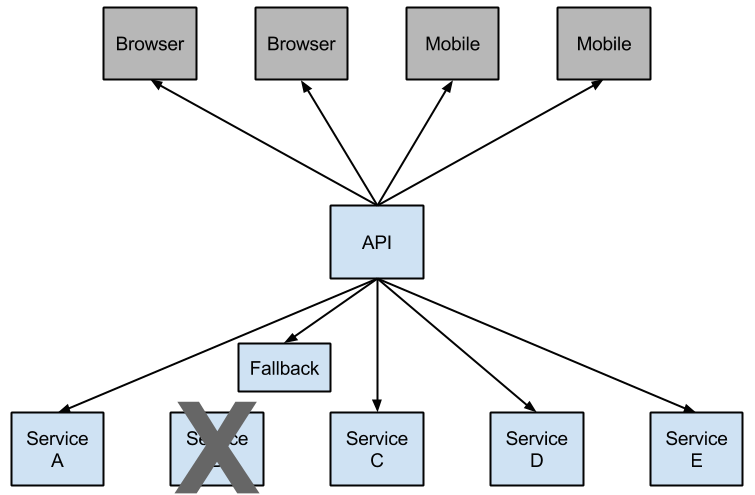
\includegraphics[height=4.2cm]{figura7}
\caption{Fallback Hystrix em falhas em cascata.}
\label{fig:figura7}
\end{figure}

\subsection{Primeiros passos com Hystrix}

Para utilizar o Hystrix, precisa ser incluso a dependência com o groupId org.springframework.cloud e o artifactId spring-cloud-starter-Hystrix, e a anotação @EnableCircuitBreaker na classe principal, conforme a figura \ref{alg:figuradez}

\begin{figure}[h]
\centering

\begin{lstlisting}[language=Java]
  @SpringBootApplication
  @EnableCircuitBreaker
  public class Application {

      public static void main(String[] args) {
          new SpringApplicationBuilder
            (Application.class).web(true)
            .run(args);
      }

  }

  @Component
  public class StoreIntegration {

      @HystrixCommand
        (fallbackMethod = "defaultStores")
      public Object getStores
        (Map<String, Object> parameters) {
          //do stuff that might fail
      }

      public Object defaultStores
        (Map<String, Object> parameters) {
          return /* something useful */;
      }
  }
\end{lstlisting}

\caption{Hystrix}
\label{alg:figuradez}
\end{figure}

No exemplo de código da figura \ref{alg:figuradez}, foi implementando uma classe que se contém um método que buscará os serviços, e para isto foi utilizado a anotação @HystrixCommand. É possível ativar as métricas Hystrix e a central de gerenciamento do mesmo adicionando as dependências conforme a figura \ref{alg:figuraonze}. O endpoint para acesso ao gerenciador é /hystrix.stream.

\begin{figure}[h]
\centering

\begin{lstlisting}[language=Java]
  <dependency>
      <groupId>
        org.springframework.boot
      </groupId>
      <artifactId>
        spring-boot-starter-actuator
      </artifactId>
  </dependency>
  <dependency>
      <groupId>
        org.springframework.cloud
      </groupId>
      <artifactId>
      spring-cloud-starter-hystrix-dashboard
      </artifactId>
  </dependency>
\end{lstlisting}

\caption{Dependencias do Gerenciados Hystrix}
\label{alg:figuraonze}
\end{figure}

\subsection{Ribbon}

Ribbon é um  balanceador de carga do lado do cliente, que fornece controles sobre o comportamento dos clientes HTTP e TCP. Uma observação importante é que a anotação @FeignClient já utiliza Ribbon, fazendo com que assim seja desnecessário a utilização do Ribbon, entretanto, quando for preciso um controle mais versátil sobre a tecnologia é optável a utilização do mesmo.

Para incluir o ribbon no projeto, será utilizado o mesmo padrão de configurações feito anteriormente. O que será alterado é o artifactId da dependência maven, que agora será utilizado spring-cloud-starter-ribbon, e para configurar o cliente Ribbon criado uma classe de configuraçao e será anotado com @RibbonClient, conforme a figura \ref{alg:figuradoze}.

\begin{figure}[h]
\centering

\begin{lstlisting}[language=Java]
  @Configuration
  @RibbonClient(name = "foo", 
    configuration = FooConfiguration.class)
  public class TestConfiguration {
  }
\end{lstlisting}

\caption{Ribbon}
\label{alg:figuradoze}
\end{figure}

\subsection{FeignClient}

FeignClient é uma biblioteca que faz com que clientes de serviços web sejam escritos de forma mais fácil. Para utilizá-lo é preciso instalar a dependência spring-cloud-starter-feign, e anotar a classe principal com @EnableFeignClients conforme a figura \ref{alg:figuratreze}. O mesmo provê suporte para anotações Spring MVC, e por utilizar o mesmo conversor de mensagens HTTP que o Spring Web, é integrada com Hystrix para fornecer um cliente com balanceamento de carga.

\begin{figure}[h]
\centering

\begin{lstlisting}[language=Java]
  @Configuration
  @ComponentScan
  @EnableAutoConfiguration
  @EnableEurekaClient
  @EnableFeignClients
  public class Application {
    public static void main(String[] args) {
        SpringApplication
          .run(Application.class, args);
    }
  }
\end{lstlisting}

\caption{FeignClient}
\label{alg:figuratreze}
\end{figure}

Ao anotar uma interface com @FeignClient conforme a figura \ref{alg:figuraquartorze}, pode ser mapeado os métodos para que consiga acesso a endpoints da biblioteca. O nome do método será qualificado e aplicado ao contexto da aplicação, fazendo com que assim não seja implementado corpo ao método pois será apenas repassados chamadas REST.

\begin{figure}[h]
\centering

\begin{lstlisting}[language=Java]
  @FeignClient("stores")
  public interface StoreClient {
    @RequestMapping(method = 
      RequestMethod.GET, 
      value = "/stores")
      List<Store> getStores();

      @RequestMapping(method = 
        RequestMethod.POST, 
        value = "/stores/{storeId}", 
        consumes = "application/json")
      Store update(
      @PathVariable("storeId") Long storeId, 
      Store store);
  }
\end{lstlisting}

\caption{Mapeamento FeignClient}
\label{alg:figuraquartorze}
\end{figure}

Cada Cliente Feign faz parte de um conjunto de componentes que trabalham juntos, para comunicar-se via HTTP. O Spring Cloud permite com que se tenha controle total sobre clientes Feign, declarando uma classe de configuração que implemente determinados métodos do FeignClient conforme a figura \ref{alg:figuraquinze}. Duas das possíveis configuração, são: modificar o padrão de Contrato que o FeignClient utiliza para que assim seja personalizado o padrão de comunicação REST que o mesmo utiliza e modificar o método de autenticação do FeignClient.

\begin{figure}[h]
\centering

\begin{lstlisting}[language=Java]
  @Configuration
  public class FooConfiguration {
    @Bean
    public Contract feignContract() {
        return new feign.Contract.Default();
    }

    @Bean
    public BasicAuthRequestInterceptor 
      basicAuthRequestInterceptor() {
      return new BasicAuthRequestInterceptor
          ("user", "password");
    }
  }
\end{lstlisting}

\caption{Autenticação com FeignClient}
\label{alg:figuraquinze}
\end{figure}

\subsection{Zuul}

Até neste capítulo, foi falado de rotas e endpoints, mas ainda não foi explorado a essencialidade de utilizar rotas. Roteamento é uma parte fundamental de uma arquitetura de micro-serviços, pelo fato de que, uma uri (identificador uniforme de recursos) pode ser mapeado de acordo com sua utilidade. Como exemplo, uma uri \/api\/usuario é mapeado para o serviço de usuário, \/api\/vendas pode ser mapeado para o serviço de vendas de uma loja. Zuul é um roteador com balanceamento de carga básico. A empresa Netflix atualmente utiliza o Zuul para os seguintes desígnios: autenticação, insights teste de stress da api, Canary test que segundo Danilo Sato \cite{danilosato2017} é uma técnica para reduzir o risco de introduzir uma nova versão de software na produção lentamente lançando a mudança para um pequeno subconjunto de usuário antes de lança-la em toda a infra-estrutura e torná-la disponível para todos, roteamento dinâmico, serviço de migração, divisão de carga, segurança, manipulação de respostas e gestão de tráfego de dados.

Para incluir o Zuul em um projeto utilizando os padrões aplicados até neste capítulo, é necessário utilizar o artifactId spring-cloud-starter-zuul, e para habilitá-lo, a classe principal deve ser anotada com @EnableZuulProxy, e este encaminhará chamadas locais para o serviço adequado. Para que de acordo com a rota seja chamado o serviço desejado deve ser configurado no arquivo de configurações principais application.yml, e para ignorar demais serviços utiliza-se a propriedade zuul.ignored-services. Na figura \ref{alg:figuradezesseis} está um exemplo da utilizaçao da mesma.

\begin{figure}[h]
\centering

\begin{lstlisting}[language=Java]
  zuul:
    ignoredServices: '*'
    routes:
    produtos: /meus-produtos/**
\end{lstlisting}

\caption{Zuul}
\label{alg:figuradezesseis}
\end{figure}

Para obter um controle mais refinado sobre determinadas rotas, pode-se especificar o caminho e o serviceId, conforme a figura \ref{alg:figuradezessete}.

\begin{figure}[h]
\centering

\begin{lstlisting}[language=Java]
  zuul:
    routes:
      produtos:
        path: /meus-produtos/**
        serviceId: produtos_service
\end{lstlisting}

\caption{Controle refinado das rotas}
\label{alg:figuradezessete}
\end{figure}

Isto significa que quando ocorrer uma chamado para a rota \"\/myprodutos\", o mesmo será encaminhado para o serviço \"produtos\_service\". Se for desejável especificar uma URL para uma localização física do serviço, pode ser feito conforme a figura \ref{alg:figuradezoito}.

\begin{figure}[h]
\centering

\begin{lstlisting}[language=Java]
  zuul:
    routes:
      produtos:
        path: /produtos/**
        url: 
        http://exemple.com/produtos_service
\end{lstlisting}

\caption{URL física do serviço}
\label{alg:figuradezoito}
\end{figure}

As configurações de rotas feitas até o momento, não são executadas como um HystrixCommand ou balancedas com Ribbon. Para conseguir isto, deve-se especificar um serviço de rota e criar um cliente Ribbon para o serviceId. Na figura \ref{alg:figuravinte} contém um exemplo de configuração para o mesmo.

\begin{figure}[h]
\centering

\begin{lstlisting}[language=Java]
  zuul:
    routes:
      produtos:
        path: /meus-produtos/**
        serviceId: produtos

  ribbon:
    eureka:
      enabled: false

  produtos:
    ribbon:
      listOfServers: exemplo.com,faype.com
\end{lstlisting}

\caption{Cliente Ribbon}
\label{alg:figuravinte}
\end{figure}

\subsection{Migração de aplicações}

Um padrão comum ao migrar um serviço Web existente, é remover endpoints antigo, e lentamente substitui-los por novas implementações. O proxy Zuul é uma ferramenta extremamente útil para isto, pelo fato de que, pode-se utilizá-lo para lidar com todo o tráfego de clientes antigos, mas lidar com solicitações para novos. Na figura \ref{alg:vinteum} contém um exemplo de configuração.

\begin{figure}[h]
\centering

\begin{lstlisting}[language=Java]
 zuul:
  routes:
    primeiro:
      path: /primeiro/**
      url: http://primeiro.exemplo.com
    segundo:
      path: /segundo/**
      url: forward:/segundo
    terceiro:
      path: /terceiro/**
      url: forward:/3rd
    legacy:
      path: /**
      url: http://teste.exemplo.com
\end{lstlisting}

\caption{Atualização de Rotas}
\label{alg:vinteum}
\end{figure}

Ao processar as solicitações de entrada, parâmetros de consulta são  decoficados para que os mesmos possam estar disponíveis para possíveis modificações nos filtro Zuul. Estes são recodificados aos reconstruir o pedido backend nos filtros de rota. O resultado pode ser diferente da entrada original, principalmente se o mesmo foi codificando utilizando por exemplo na linguagem Javascript a função encodeURIComponent(). Isto não causa problemas na maiorias dos casos, entretanto, algumas aplicações web podem exigir codificação de url para consultas complexas. Para forçar a codificação original da url, é possível utilizar a configuração zull.forceOriginalQueryStringEncoding definindo-à como true.


\subsection{RxJava com Spring MVC}

RxJava é uma implementação Java VM de extensões reativas : uma biblioteca para compor programas assíncronos e baseados em eventos utilizando sequências observáveis \cite{reactivex2017}.

Spring Cloud fornece suporte para observables que em RxJava é um objeto que implementa a interface Observable que em seguida, este assinante reage a qualquer item ou sequência de itens que o objeto Observable emite. Esse padrão facilita operações simultâneas porque não precisa bloquear enquanto espera que o Observable emita objetos, mas ao invés disto, cria uma sentinela na forma de assinante que está pronto para reagir apropriadamente em qualquer tempo futuro que o Observable gere \cite{reactivex2017}. Utilizando o Spring Cloud pode-se retornar objetos rx.Single, rx.Observale e SSE (Eventos enviados pelo servidor) que é uma tecnologia pelo qual um navegador recebe atualizações de um servidor via HTTP. Na figura \ref{alg:vintedois} está dois exemplos, segundo a Netflix \cite{netflix2017SpringCloud} de como utilizá-los.

\begin{figure}[h]
\centering

\begin{lstlisting}[language=Java]
  @RequestMapping(method =
    RequestMethod.GET, value = "/multiple")
    public Single<List<String>> multiple() {
      return Observable
        .just("multiple", "values")
        .toList().toSingle();
  }

  @RequestMapping(
      method = RequestMethod.GET, 
      value = "/responseWithObservable")
  public ResponseEntity<Single<String>> 
      responseWithObservable() {

  Observable<String> observable = 
  Observable.just("single value");
  HttpHeaders headers = new HttpHeaders();
  headers
    .setContentType(APPLICATION_JSON_UTF8);
  return new ResponseEntity<>(
        observable.toSingle(), 
      headers, HttpStatus.CREATED);
  }
\end{lstlisting}

\caption{Compilação do firmware}
\label{alg:vintedois}
\end{figure}

\subsection{Motivação de uso das tecnologias apresentadas}

Até o prezado momento, foram apresentados diversas tecnologias, entretanto, fica a questão sobre o por que de tantas tecnologias. e a resposta é clara e objetiva. Para que se tenham micro-serviços, é necessário a utilização de um recurso para a orquestração dos mesmos, neste caso, entra o Eureka. Quando se tem micro-serviços, é necessário a centralização dos mesmos para que não fique espalhados e perdidos em hosts ou portas diferentes, surge a necessidade de um gateway, neste caso, o Zuul. A partir do momento que são integrados muitos micro-serviços, torna-se difícil o gerenciamento da configuração dos mesmos, surgindo a necessidade de um mecanismo para fácil configuração e integração de aplicações, por isto, foi apresentado o Spring Config. Após tudo isto, surge ainda um problema, o balanceamento de carga, um problema abrangente quando se trabalha com aplicações distribuidas. Surge então, a motivação de utilizar o Ribbon para distribuição de carga. Com tudo isto configurado, ainda não se tem garantia precisa de disponibilidade da aplicação, fazendo com que, se caso ocorrer um problema em um micro-serviço, necessite de uma tecnologia que resolva esta questão, fazendo assim necessário a utilização do Hystrix. A motivação de apresentar tecnologias Spring Cloud e Netflix, como citado na introdução deste trabalho, é o fato da experiência e sucesso por parte dos mesmos em aplicações distribuidas.


\section{Resultados}

Desenvolver uma estrutura utilizando micro-serviços pode ser trabalhoso, quando se tem muitos serviços para gerenciar se torna um processo complexo. Entretanto, existem diversas ferramentas que auxiliam neste processo. Durante este trabalho, foram feitos diversos testes, utilizando ferramentas da empresa Netflix para auxílio no processo de desenvolvimento de micro-serviços. Foi utilizado ferramentas para registro de micro-serviços, balanceamento de carga e tolerância a falhas. Em todos foi obtido resultados e têm funcionado da forma esperada.

\section{Conclusões e trabalhos futuros}

Conclui-se portanto, que é possível criar uma estrutura utilizando micro-serviços, e que existem dificuldades ao gerenciar este estrutura, quando existem muitos micro-serviços envolvidos. Mas utilizando-se de ferramentas para auxílio no desenvolvimento desta estrutura, torna-se possível a criaçao da mesma. Quando é utilizado esta estrutura, os sistemas são mais tolerantes a falhas pelo fato de que, se um serviço parar, os demais continuam. Um ponto a ser levantado, é que as aplicações possuem alta coesão e baixo acoplamento, o que facilita no gerenciamento das mesmas.

\appendices
\section{Proof of the First Zonklar Equation}
Appendix one text goes here.

% you can choose not to have a title for an appendix
% if you want by leaving the argument blank
\section{}
Appendix two text goes here.


% use section* for acknowledgment
\section*{Acknowledgment}


The authors would like to thank...


% Can use something like this to put references on a page
% by themselves when using endfloat and the captionsoff option.
\ifCLASSOPTIONcaptionsoff
  \newpage
\fi

\begin{thebibliography}{1}

\bibitem{tecnetflixhipsters}
Paulo Silveira. Mauricio Balboa Linhares. \emph Tecnologias na Netflix. 2017 [Online] Disponível: http://content.blubrry.com/hipsterstech/hipsters\_041\_netflix.mp3. [Acesso: 25-Abr-2017]

\bibitem{flaviosilveira}
Flavio Silveira. \emph Microserviços - O que é? 2016 [Online] Disponível:
http://flaviosilveira.com/2016/microservicos. [Acesso: 06-Mai-2017]

\bibitem{CleutonSampaio}
Cleuton Sampaio. \emph Micro serviços: O que são e para que servem. 2015 [Online] Disponível: http://www.obomprogramador.com/2015/03/micro-servicos-o-que-sao-e-para-que.html. [Acesso: 28-Fev-2017] 

% TODO DEVE SER RETIRADO E SUBSTITUIDO PELA FONTE MARTIN FLOWER
\bibitem{JamesLewis}
James Lewis. (2016). \emph Microsserviços em poucas palavras. [Online] Disponível: https://www.thoughtworks.com/pt/insights/blog/microservices-nutshell. [Acesso: 20-Mar-2017]

\bibitem{AdrianoAlmeida}
Adriano Almeida. \emph Arquitetura de microserviços ou monolítica. 2015 [Online] Disponível: http://blog.caelum.com.br/arquitetura-de-microservicos-ou-monolitica. [Acesso: 22-Mar-2017]

\bibitem{CristianoDiedrich}
Cristiano Diedrich. \emph O que é Docker. 2015 [Online] Disponível: http://www.mundodocker.com.br/o-que-e-docker. [Acesso: 01-Dez-2016]

\bibitem{JanStenberg}
Jan Stenberg. \emph O estado da arte em micro serviços. 2015 [Online] Disponível: https://www.infoq.com/br/news/2015/04/microservices-current-state. [Acesso: 08-Fev-2017]

\bibitem{RicardoPeloi}
Ricardo Peloi. \emph Como implantar uma verdadeira Arquitetura de Microserviços na sua empresa. 2016 [Online] Disponível: http://sensedia.com/blog/soa/implantar-arquitetura-de-microservicos. [Acesso: 08-Mar-2017]

\bibitem{ChrisRichardson}
Chris Richardson. \emph Whois using microservices. 2016 [Online] Disponível: http://microservices.io/articles/whoisusingmicroservices.html. [Acesso: 20-Mai-2017]

\bibitem{idc2017}
IDC. \emph Connecting the IotT: The road to success. 2016 [Online] Disponível: http://www.idc.com/infographics/IoT. [Acesso: 15-Fev-2017]

\bibitem{martinfowleretal}
Martin Fowler et al. \emph Microservices. 2014 [Online] Disponível: https://www.martinfowler.com/articles/microservices.html. [Acesso: 20-Mai-2017]

\bibitem{netflix2016Ribbon}
Netflix. \emph Ribbon. 2016 [Online] Disponível: https://github.com/Netflix/ribbon/wiki. [Acesso: 06-Mai-2017]

\bibitem{netflix2016Zuul}
Netflix. \emph Zuul. 2016 [Online] Disponível: https://github.com/Netflix/zuul/wiki. [Acesso: 02-Mai-2017]

%% TODO ONDE TA???
\bibitem{martinfowler2017CircuitBreaker}
Martin Fowler. \emph CircuitBreaker. 2014 [Online] Disponível: https://martinfowler.com/bliki/CircuitBreaker.html. [Acesso: 02-Mar-2017]

\bibitem{danilosato2017}
Danilo Sato. \emph CanaryRelease. 2014 [Online] Disponível: https://martinfowler.com/bliki/CanaryRelease.html. [Acesso: 10-Abr-2017]

\bibitem{netflix2017SpringCloud}
Netflix. \emph Spring Cloud Netflix. 2016 [Online] Disponível: http://cloud.spring.io/spring-cloud-netflix/spring-cloud-netflix.html. [Acesso: 18-Dez-2016]

\bibitem{nicoladragonietal}
Nicola Dragoni et al. \emph Microservices: yesterday, today, and tomorrow. Technical University of Denmark, vol 1, pp. 1-3, 2016

\bibitem{willianmunif}
Willian Marques Freire. Munif Gebara Junior. \emph Artigo IoT - Internet das coisas. vol 1, pp.1-3, 2017

\bibitem{reactivex2017}
ReactiveX. \emph Observable. 2015 [Online] Disponível: http://reactivex.io/documentation/observable.html. [Acesso: 25-Nov-2016]

\end{thebibliography}


\begin{IEEEbiography}[{
\includegraphics[width=1in,height=1.25in,clip,keepaspectratio]{willian}}]{Willian Marques Freire}
Possui Ensino Médio completo pelo Colégio Estadual Rosa Delúcia Calsavara (2013). Atualmente é Desenvolvedor de Software da Gumga Tecnologia da Informação S/A. Tem experiência na área de Ciência da Computação.
\end{IEEEbiography}

\begin{IEEEbiography}[{
\includegraphics[width=1in,height=1.25in,clip,keepaspectratio]{munif}}]{Munif Gebara Júnior}
Possui graduação em Ciência da Computação pela Universidade Estadual de Maringá (1997) e mestrado em Engenharia Elétrica e Informática Industrial pela Universidade Tecnológica Federal do Paraná (2001). Atualmente é professor da Fundação Faculdade de Filosofia Ciências e Letras de Mandaguari e professor de ensino superior da Faculdade de Tecnologia e Ciências do Norte do Paraná Ltda e desenvolvedor.
\end{IEEEbiography}

\end{document}


